\chapter{MammoDetect System}
\label{chap:ch5}

\section{Functionalities}
The system consists of two main functionalities: selecting an image, either from the array of examples provided in the top right corner of the interface, or the upload button, which opens the computer's internal storage. Upon selecting an image, it will be viewed in the main window. The image selected does not necessarily have to be 512$\times$512 because it will be resized anyway. The user then has the choice of either selecting another image or submitting the image to the model to be classified into normal and cancerous, the latter being then sent to the detection model to replace the image in the main window with the same image that has drawn the bounding box resulted from passing the image to the model. 

The detection model also classifies the tumors as benign or malign. In the bottom right corner, below the examples image array, there are two boxes. The top one contains the top two classes the models classified the image as, while the bottom one displays the true label of the image, if it was selected from the examples array. If the image has not been selected from the examples array, the bottom box will contain the word "unknown".

Because the way this library sends the data from the image selected doesn't include the actual name of the filename, I found myself thinking of ways to find and display the true label of the images selected from the examples. To do so, I compared the contents of each of the images existing in the directory to the contents of the image selected. In preparation for this, for each image saved as index.png, index being a variable from 1 to 151, I saved an additional file named index-label.txt, where label is either 0 or 1, corresponding to the labels normal or cancer. For the images uploaded from the user's device, there is no way to find the true label of the input; therefore, I added another class, unknown, that is displayed whenever the label of the image cannot be determined.

Comparatively, if the image is detected to be normal, the main window will not change, instead displaying the original image.

\section{Design}

Figure \ref{fig:fig38} shows the architecture diagram. Figure \ref{fig:fig39} shows the class diagram. The Fitter class is used to train the detection model; the classification model is trained in a simple loop. Figure \ref{fig:fig40} shows the sequence diagram.

\begin{figure}[H]
    \centering
    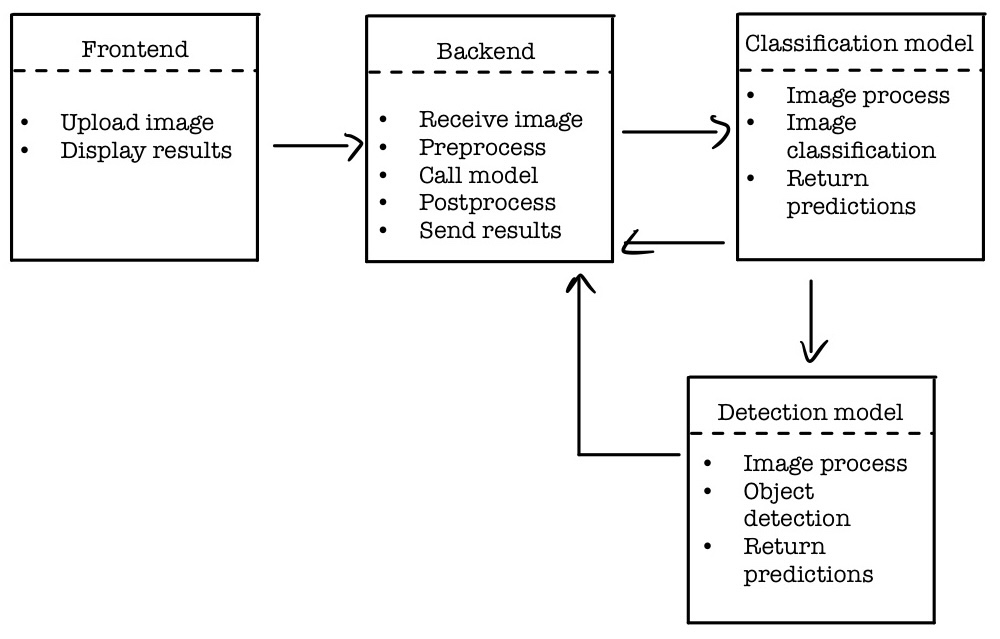
\includegraphics[width=0.5\linewidth]{figures/Figure50.png}
    \caption{System architecture diagram}
    \label{fig:fig38}
\end{figure}

\begin{figure}[H]
    \centering
    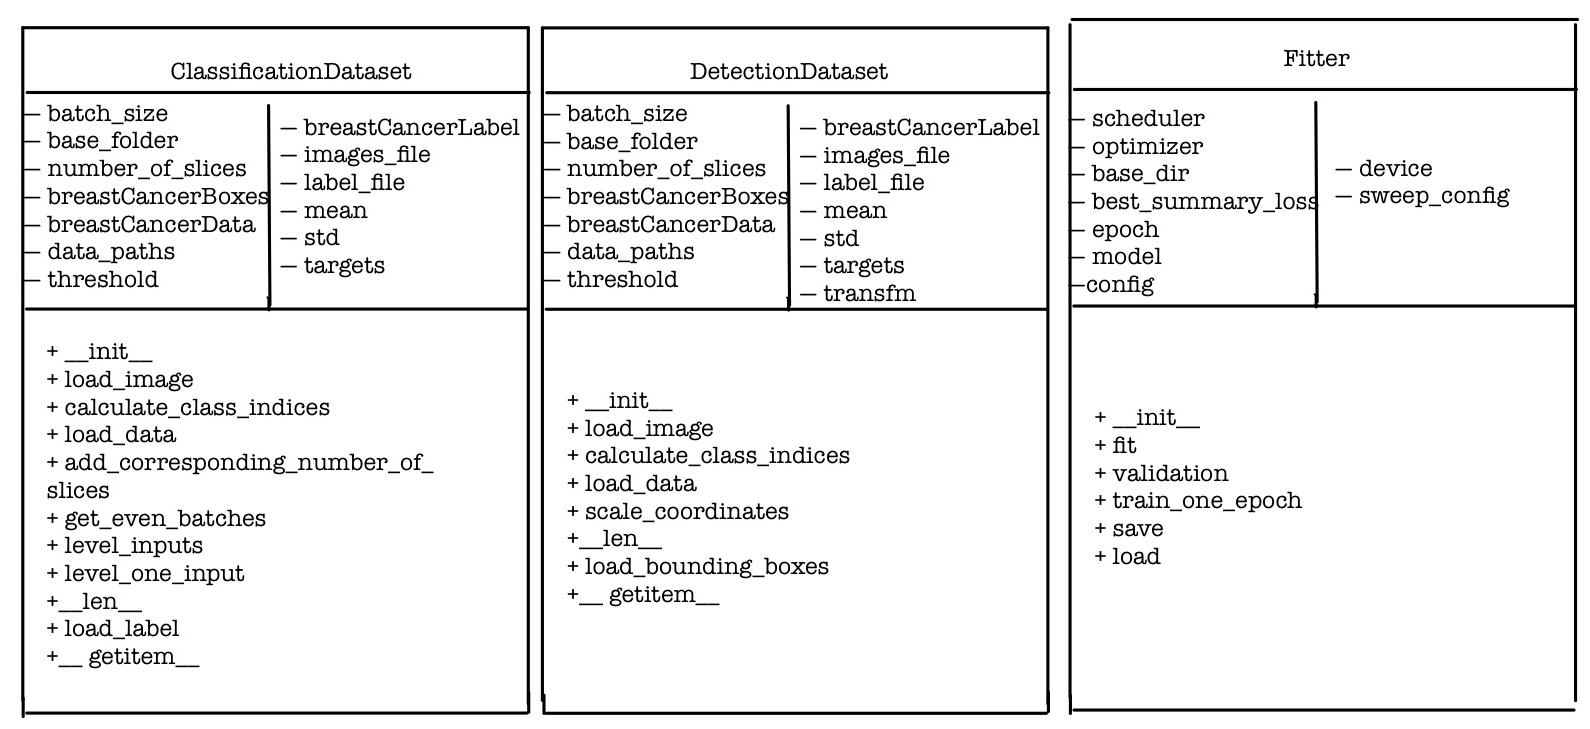
\includegraphics[width=0.5\linewidth]{figures/Figure51.png}
    \caption{System class diagram}
    \label{fig:fig39}
\end{figure}

\begin{figure}[H]
    \centering
    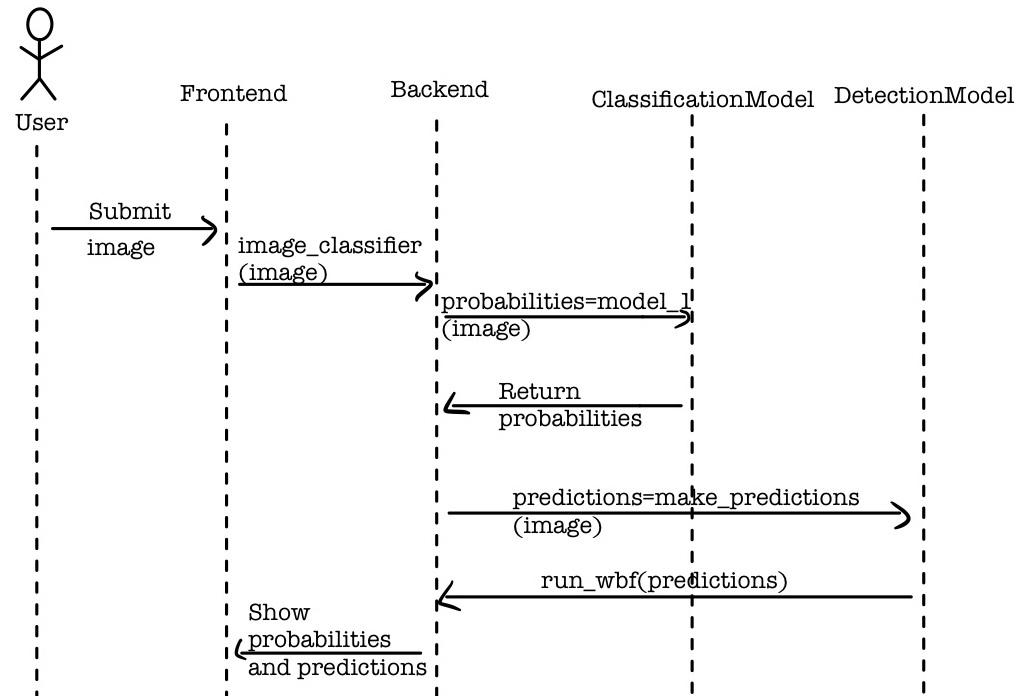
\includegraphics[width=0.5\linewidth]{figures/Figure52.png}
    \caption{System sequence diagram}
    \label{fig:fig40}
\end{figure}

\section{Implementation}
Both the train and front-end sections of the system were implemented in Python. For the front-end, I used the library Gradio. First, I used the Gradio Interface method of creating a GUI; however, I did not like that the examples array was out of view when uploading an image of 512$\times$512. This can be seen in image \ref{fig:fig15}.

\begin{figure}[H]
    \centering
    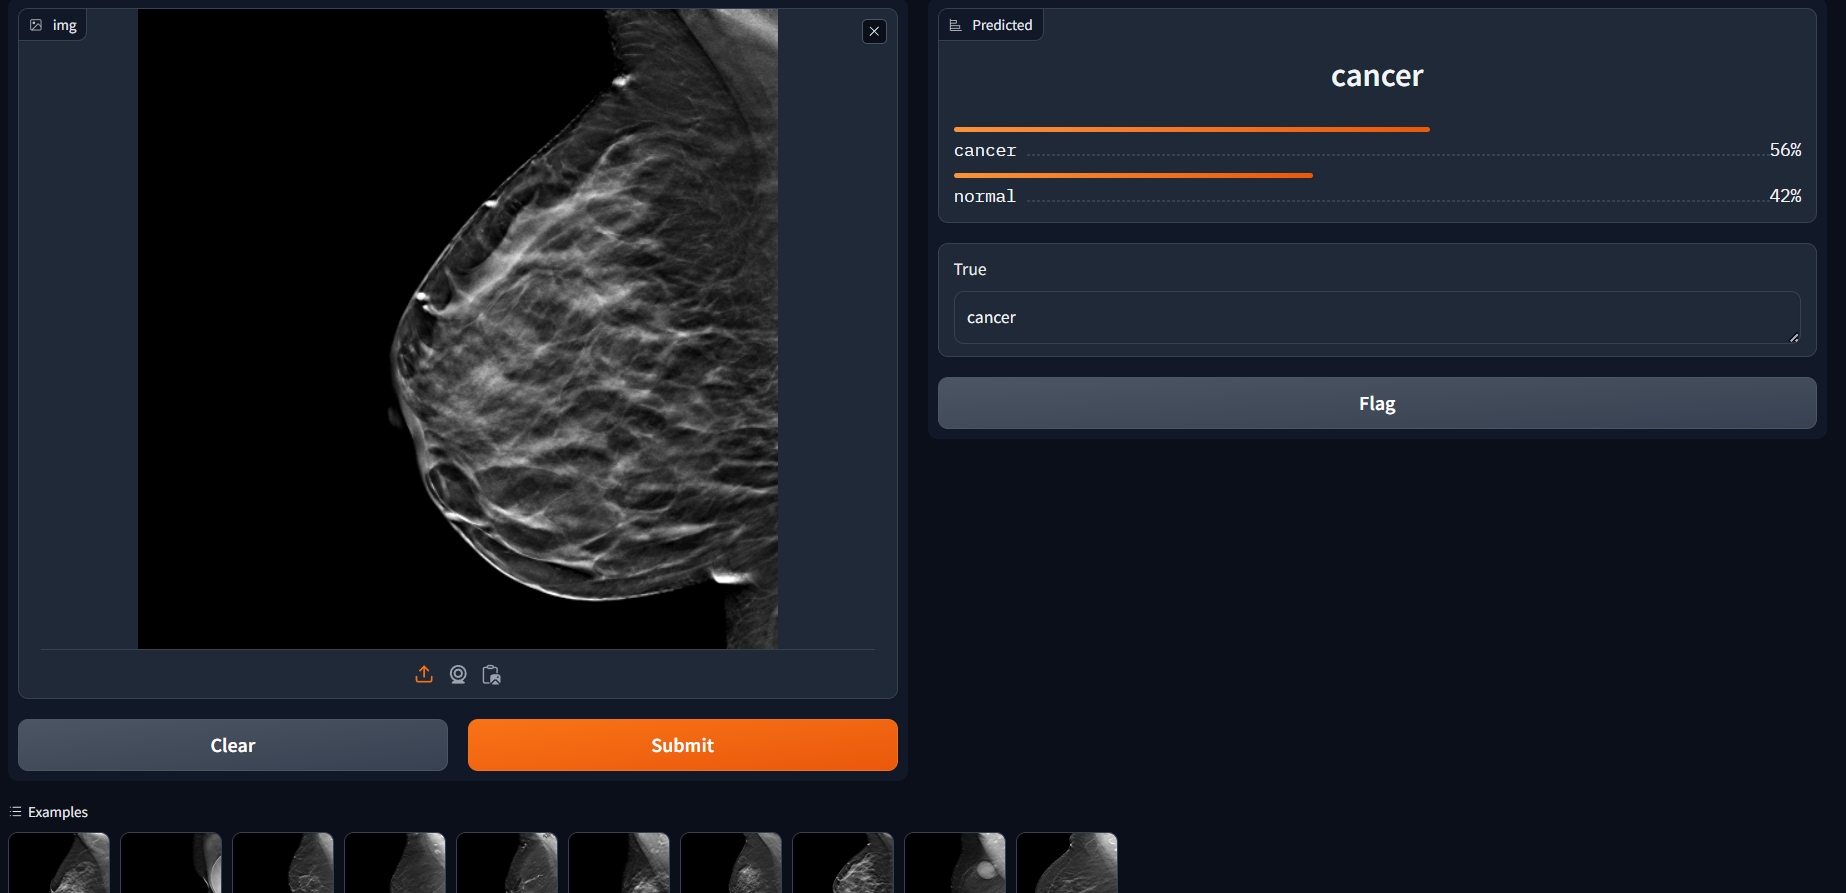
\includegraphics[width=0.75\linewidth]{figures/Figure16.png}
    \caption{Application interface}
    \label{fig:fig15}
\end{figure}

Then, I experimented with the Gradio Blocks method and I also chose a theme to go with the system. Figure \ref{fig:fig37} show how the interface looked with no image selected and how it looked after submitting.

\begin{figure}[H]
    \subfigure[No image selected]{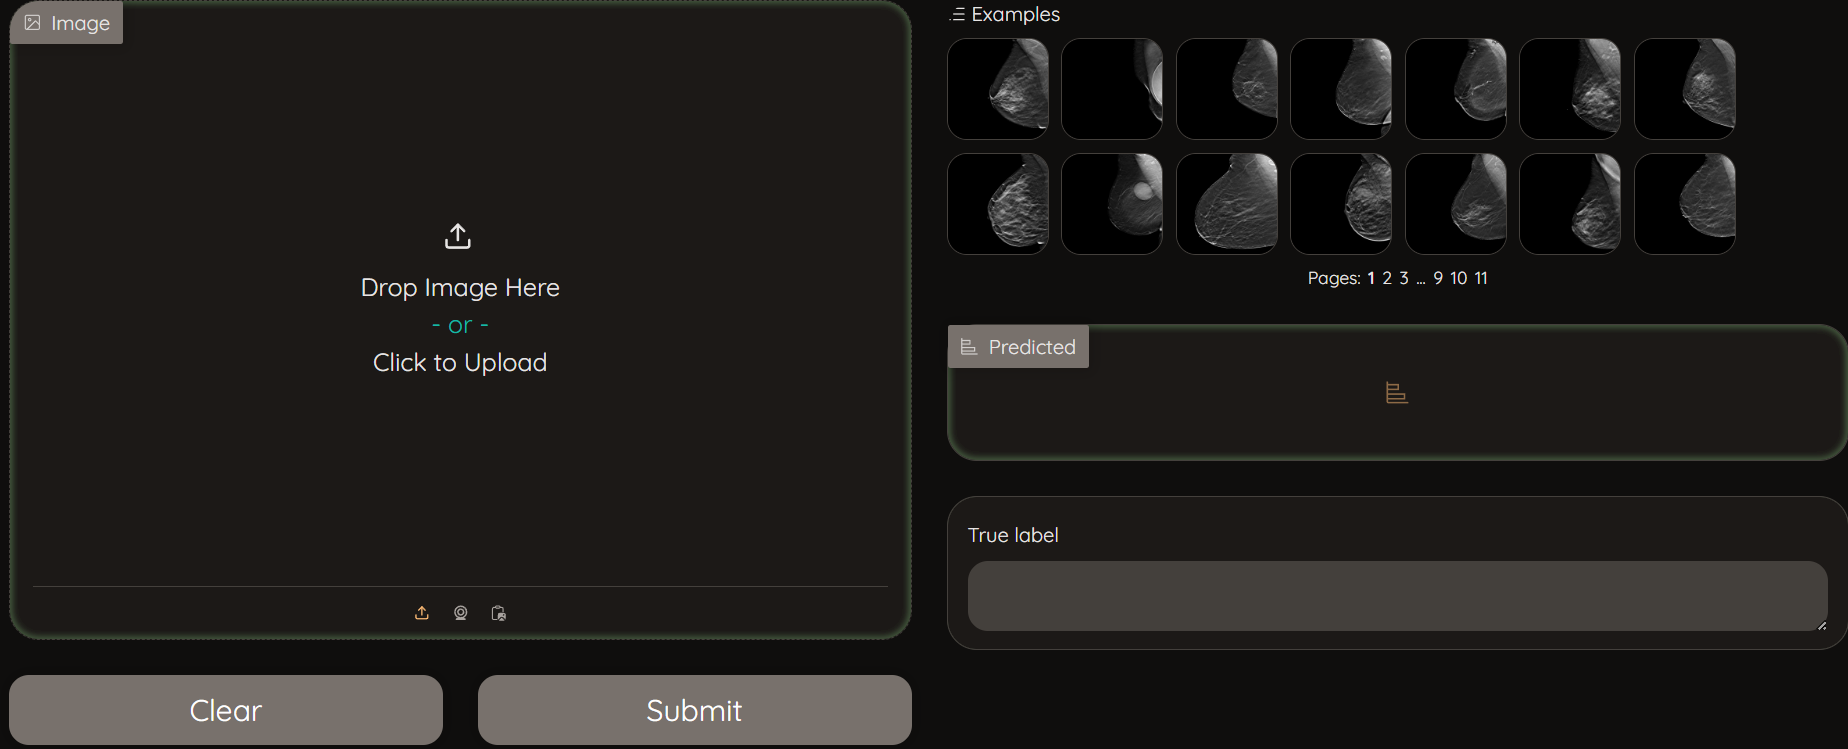
\includegraphics[width=0.5\linewidth]{figures/Figure48.png}}
    \subfigure[Image selected and submitted]{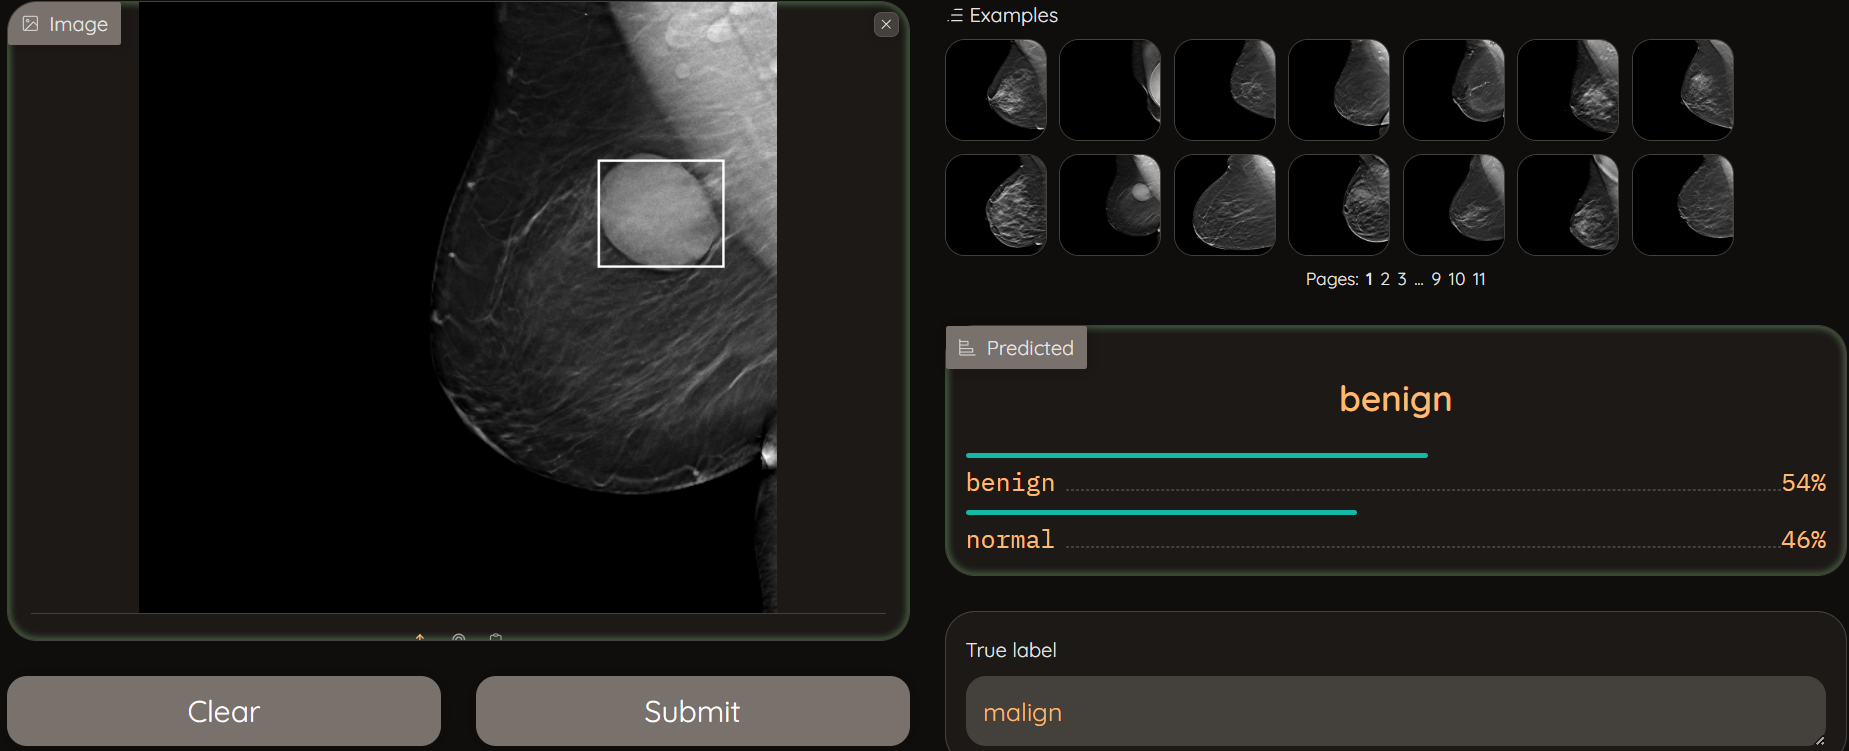
\includegraphics[width=0.5\linewidth]{figures/Figure49.png}}
    \caption{GUI}
    \label{fig:fig37}
\end{figure}

The models' architecture used was the one in the Torch library. I implemented my own datasets for both the classification and detection problems that inherit methods from $torch.utlis.data.Dataset$. The order of the inputs so that each batch is balanced is determined directly in the dataset classes, so the $torch.utils.data.DataLoader$ does not take any sampler classes as input, instead setting the $shuffle$ attribute to False. The batch size is sent to both the DataLoader and Dataset classes.

\section{Testing and validation}

In order to make sure that the system behaved accordingly, I tested the function \textit{find\_image\_path} from the directory \textit{utils}, used in the $\_\_getitem()\_\_$ function in both datasets. This method is supposed to remove the name of the file at the end of a long string representing the path to the dcm files and add the string "NA-" in the last directory name after the "-". The reason this method exists is that the png images are saved in directories with the same name as the dcm files. Also, the name of the files contains the string mentioned before; this might be because I downloaded the dcm files before the latest update of the dataset, which was in January 2024.

For testing this method, I used some simple assertions to make sure that the function was fulfilling its intended use.